\documentclass[11pt,a4paper]{article}
\usepackage[left=2cm,right=2cm,top=2cm,bottom=3cm]{geometry}
\usepackage{amsmath,amsfonts,amsthm,amssymb,varioref,times, commath}
\usepackage{gensymb}
\usepackage{tikz}
\usepackage{textcomp}
\usepackage{hyperref}
\hypersetup{
 colorlinks=true,
 linkcolor=blue,
 filecolor=magenta, 
urlcolor=cyan,
}
\usepackage{lipsum}
\usepackage{epigraph}
%to resume numbering in a list
\usepackage{enumitem}
%----- arrows 
\usepackage{extarrows}

%    differential equatiosn 
\usepackage{diffcoeff}   %\diff[2]{x}{y}


%%%%%%pour ecrire en français avec les accents
\usepackage[utf8]{inputenc}
\usepackage[T1]{fontenc}
\usepackage{lmodern} % load a font with all the characters
\usepackage{units}
%%%%%%%Image-related packages
\usepackage{wrapfig}
\usepackage{float, graphicx}
\graphicspath{ {./img/} }
\usepackage{subcaption}
\usepackage[export]{adjustbox}

%%%%%%%pour faire des cadres
\usepackage{xcolor}
\usepackage{tcolorbox}
\usepackage{framed}
\usepackage{mdframed}


%%%%%%%chemistry frmulae
\usepackage{chemfig}
\usepackage{chemformula}
\usepackage[version=4]{mhchem}

% -------------- Circuits -------------------
\usepackage[european, straightvoltages]{circuitikz}

% Title & headers
\usepackage[explicit]{titlesec}
% Raised Rule Command:
% Arg 1 (Optional) - How high to raise the rule
% Arg 2 - Thickness of the rule
\newcommand{\raisedrulefill}[2][0ex]{\leaders\hbox{\rule[#1]{1pt}{#2}}\hfill}
\titleformat{\section}{\Large\bfseries}{\thesection. }{0em}{#1\,\raisedrulefill[0.4ex]{1pt}}

% pour ecrire sur +sieurs colonnes
\usepackage{multicol}
\setlength{\columnseprule}{0pt}
\setlength{\columnsep}{60pt}
% Fusion de lignes de tableaux.
\usepackage{multirow}
% Position verticale des lettres dans la ligne de tableau.
\usepackage{array}

% physics -----------------------------------------------------------
\newcommand{\To}{\longrightarrow}
\newcommand{\gpl}{\; g\cdot L^{-1}}
\newcommand{\gpmol}{\; g\cdot mol^{-1}}
\newcommand{\mpl}{\; mol\cdot L^{-1}}
\newcommand{\mps}{\; m\cdot s^{-1}}
\newcommand{\rps}{\; rad\cdot s^{-1}}
\newcommand{\kph}{\; km\cdot h^{-1}}
\newcommand{\mpss}{\; m\cdot s^{-2}}
\newcommand{\Dt}{\Delta t}
\newcommand{\vv}{\vec{v}}
\newcommand{\va}{\vec{a}}
\newcommand{\vp}{\vec{p}}
\newcommand{\vf}{\vec{F}}
\newcommand*{\Vf}[1]{\overrightarrow{F_\ensuremath{{#1}}}}
\newcommand{\es}[1]{\cdot10^{#1}}
\newcommand{\eng}[1]{\textcolor{purple}{(= #1})}
\usepackage{harpoon}
%\newcommand*{\vect}[1]{\overrightharp{\ensuremath{#1}}}
\newcommand*{\Vect}[1]{\overrightarrow{\ensuremath{#1}}}
\newcommand{\pfd}[1]{\sum \vec{F}_{ext_{#1}} &= \od{\vp_{#1}}{t} = m\cdot\va_{#1}}
\newcommand{\C}{\degree C}
\newcommand{\Delt}{\Delta t}

% --- Circuits ------------
\newcommand{\bipole}[1]{
\begin{circuitikz} \draw
(0,0) to[ #1 ] (2,0); 
\end{circuitikz} {\hspace{5mm}}}

% Chimie ---------------------------------
\newcommand{\oxo}{\ce{H3O+}_{(aq)}}
\newcommand{\eau}{\ce{H2O}_{(\ell)}}
\newcommand{\OH}{\ce{HO-}_{(aq)}}
\newcommand{\AH}{\ce{AH}_{(aq)}}
\newcommand{\A}{\ce{A-}_{(aq)}}
\newcommand{\MnO}{\ce{MnO_4^{-}}}
\newcommand{\conc}[1]{\left[{#1}\right]}
\newcommand{\couple}[2]{\ce{#1/#2}}


% Environnements ------------------------
\newcounter{exo}
\newenvironment{exo}[1][]
{\refstepcounter{exo} \begin{shaded}\noindent $\triangleright \quad$\textbf{Exercice~\theexo. #1} } { \end{shaded}}
\newenvironment{eg}
{\begin{shaded} \textbf{Exemple:} } { \end{shaded}}

\newenvironment{defn}[1]
{\begin{leftbar}\noindent \textbf{Définition :\textit{ \quad #1}} } { \end{leftbar}}

%\newenvironment{rmrq}
%{\begin{shaded} \textbf{Remarque.\quad } \itshape } { \end{shaded}}
\newenvironment{rmrq}
{\begin{mdframed}[backgroundcolor=blue!10, linewidth=0pt] \textbf{Remarque.\quad } \itshape } { \end{mdframed}}

\newenvironment{python}
{\begin{shaded} \textbf{A faire en PYTHON}\\ \itshape } { \end{shaded}}

% Shading colour -----------------------------
\definecolor{shadecolor}{gray}{0.9}

\date{}
\author{}

\renewcommand*\contentsname{Résumé}









% parametres des entete et de pieds de pages
\usepackage{fancyhdr}
\pagestyle{fancy}
\fancyhf{}
\lhead{SciPhy : Terminale spé}
\rhead{$\chi $ -  2bis : Piles}
\chead{2020-28}
\rfoot{Page \thepage}
\lfoot{\textcopyright\; S Zayyani}


\title{\large Chimie - Chapitre 2 bis \\ \LARGE  Les piles électrochimiques \\}

\setlength{\parindent}{0mm}
\setlength{\parskip}{2mm}

%%%%%%%%%%% For wrapfigure 
\setlength{\intextsep}{6pt}%
\setlength{\columnsep}{3pt}%


\begin{document}
\maketitle
\vspace{-1cm}

\begin{tcolorbox}[title=Notions de la classe de première à rappeler]
Tableaux d'avancement ; avancement chimique ; couples rédox ; réactions d'oxydoréduction
%\tcblower
\end{tcolorbox}
\tableofcontents

\section{Pile : Le principe}
Allons droit au but : une pile \eng{battery} est une réaction rédox où les électrons échangés passe par l'intermédiaire d'un dipôle, placé entre les deux couples. 

Normalement dans une réaction d'oxydoréduction, il y a un ou plusieurs électrons échangés entre le réducteur d'un couple et l'oxydant de l'autre couple. Cet échange a lieu directement dans le milieu réactionnel. 

Si l'on impose que les électrons libérés par l'oxydation du réducteur passent d'abord par un dipôle, à l'extérieur, nous avons construit une pile électrochimique. 


\section{Pile : Composition}

La pile, étant une réaction rédox entre deux couples, est composé de deux \textbf{demi-piles}. 
Chaque demi-pile est composée d'un oxydant et de son réducteur, en forme \textbf{d'une plaque métallique (l'électrode) plongée dans une solution contenant le cation du métal} (e.g. une plaque de cuivre dans une solution contentant des ions $\ce{Cu^2+}$). Chaque demi-pile est donc relative à un des couples rédox de la pile. 

Les deux demi-piles sont reliées d'un coté par une \textbf{jonction électrochimique}, ou \textbf{jonction} \eng{junction} tout court. Cette jonction est souvent un \textbf{pont salin} \eng{salt bridge}, un tube en $U$ qui contient une solution électrochimique gélifiée contenant des ions qui peuvent migrer, et donc établir un courant électrique entre les demi-piles, sans mélange entre espèces en solution. La présence du pont salin est essentielle pour la fermeture du circuit électrique, et le fonctionnement de la pile. 

\begin{figure}[h]
    \centering
    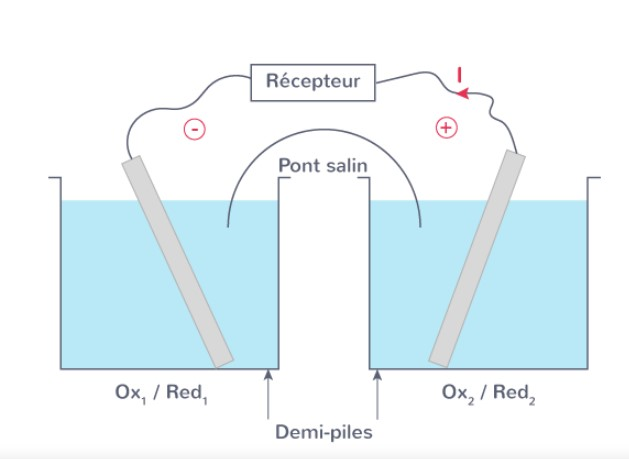
\includegraphics[width=0.7\linewidth]{imgs/c2bis/pile1.jpg}
    \caption{Schéma général d'une pile électrochimique}
\end{figure}

Finalement, là où nous branchons la pile sur le dipôle s'appelle le circuit extérieur. On y trouve les deux bornes de la pile, notées souvent $(+)$ et $(-)$. Tant que la résistance dans le circuit extérieur n'est pas trop grand, une réaction a lieu entre les deux demi-piles, et la pile débitera un courant électrique.

\section{Pile : Fonctionnement}

Le sens du courant (conventionnel) du courant est de la borne $(+)$ vers la borne $(-)$, ce qui implique que les électrons font le parcours inverse. 

L'oxydation libère des électrons, et donc les électrons doivent commencer leur parcours dans l'électrode qui est le \textbf{siège de l'oxydation}, nommée l'\textbf{anode}. L'autre électrode, \textbf{siège de la réduction}, où se trouve les électrons à la fin de leur parcours, se nomme \textbf{cathode}. 

La réaction de la pile, donc, est la somme de la réaction de réduction à la cathode, et la réaction d'oxydation à l'anode. L'équation de cette réaction, est exactement comme les équations de rédox que vous avez déjà vues, c'est à dire, il n'y a rien dans l'écriture pour indiquer qu'il s'agit d'une pile. 

\begin{eg}
La pile Daniell, inventée en 1836, est entre les couples $\ce{Cu^2+/ Cu}$ et $\ce{Zn^2+/ Zn}$. 

La cathode a pour réaction : $\ce{Cu^2+_(aq) + 2e- -> Cu_(s)} $ \\
L'anode a pour réaction : $\ce{Zn_(s) -> Zn^2+_(aq) + 2e-} $

La réaction de la pile est donc : $\ce{Cu^2+_(aq) + Zn_(s) -> Zn^2+_(aq) + Cu_(s)} $
\end{eg}


\begin{figure}[ht]
\centering
\begin{subfigure}{.45\textwidth}
  \centering
%%%%%%%%%%%%%%%  % include second image
  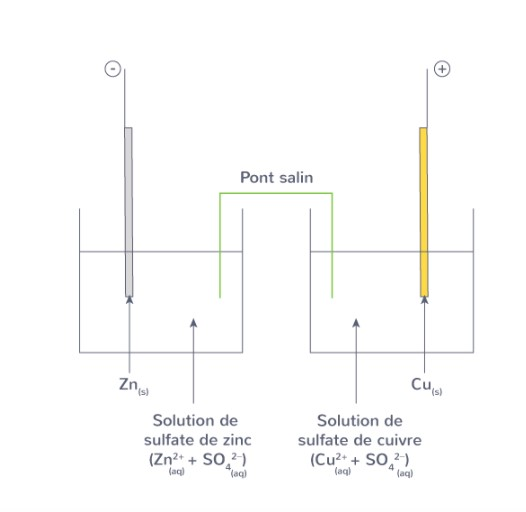
\includegraphics[width=.95\linewidth]{imgs/c2bis/dnaiell1.jpg}  
\end{subfigure}
\begin{subfigure}{.45\textwidth}
  \centering
  %%%%%%%%%%%%%% include second image
  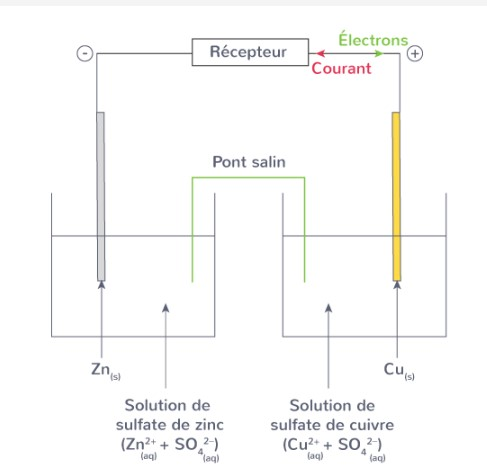
\includegraphics[width=.95\linewidth]{imgs/c2bis/daniell2.jpg}  
\end{subfigure}
\caption{Schéma d'une pile Daniell.}
\end{figure}

\begin{rmrq}
Il est essentiel de comprendre qu'une pile qui fonctionne est une système chimique \textbf{hors équilibre}. Pour que la pile fonctionne, il faut que la réaction rédox entre les couples mis en jeu avance dans le sens direct. Comme toute réaction chimique limitée, cette réaction est caractérisée par une constante d'équilibre $K$. L'état de la réaction à un instant donné est caractérisé, à son tour, par le quotient de la réaction $Q$. 

Tant que la pile débite, la réaction avance dans le sens direct, c'est à dire $Q\neq K$, et plus précisément $Q<K$. 

Plus $Q$ tend vers $K$, plus la réaction tend vers l'équilibre, et donc sa fin. Une fois $Q = K$, la réaction s'arrête : la pile est usée. 

Dans le case des accumulateurs (piles rechargeables), nous pouvons forcer la réaction dans le sens inverse, afin de re-établir le déséquilibre du départ: ils s'agit d'une \textit{évolution forcée}, que l'on verra plus tard. 
\end{rmrq}

\section{Pile : Caractéristiques}

La caractéristique principale d'une pile (selon laquelle souvent nous choisissons la pile) s'appelle 
sa force électromotrice. 
\begin{defn}{Force électromotrice}

La force électromotrice d'une pile, souvent notée $fem$ ou $E$, est la valeur absolue de la tension entre les bornes d'une qui ne débite pas. Elle s'exprime en volts ($V$). 
\end{defn}

\begin{rmrq}
Il est important de noter que, malgré son appellation, la force électromotrice \textit{n'est pas} une force. C'est une tension, d'où les unités en volts. 

La valeur de la $fem$ d'une pile dépénd de sa composition, c'est à dire, de la concentration, et de la nature des couples rédox qui la constituent. 
\end{rmrq}

\begin{eg}
L'écriture symbolique d'une pile est de façon suivante (dans le cas de la pile Daniell): 
$$(-)\ce{Zn_{(s)}/Zn^2+_{(aq)} // Cu^2+_{(aq)} / Cu_{(s)}}(+) $$ 
\end{eg}


\section{Pile : Capacité}

\begin{defn}{Capacité d'une pile}
\begin{itemize}
    \item La \textbf{quantité d'électricité débité} par une pile, pendant la durée $\Delta t$, et délivrant une intensité de courant $I$ est : 
    $$ Q = I\cdot \Delta t  \quad avec \quad \begin{cases}
    I \rightarrow  \text{intensite du courant en }(A) \\
    \Delta t \rightarrow \text{ durée de fonctionnement en }(s) \\ 
    Q \rightarrow  \text{charge débitée en }(C)
     \end{cases}$$
    \item La \textbf{capacité} d'une pile, est la \textbf{quantité maximale} de charge $Q_{max}$ débitée par une pile, entre l'instant initial où la réaction rédox de la pile a été déclenchée, et l'état final, où la réaction atteint son état d'équilibre. 
    \item Le charge débité s'exprime en coulombs (C), en SI, mais souvent, on l'exprime aussi en ampère-heure $(A\cdot h$), où milliampère-heure $mA\cdot h$ (comme pour la capacité des batteries dans les téléphones portables). 
\end{itemize}
\end{defn}

Nous pouvons aussi exprimer la capacité d'une pile, en termes de quantités de réactifs et de nombre d'électrons échangés. La nouvelle définition de la capacité d'une pile est donc : 

\begin{shaded}
$$ Q = z\cdot x_f\cdot F  \quad avec \quad \begin{cases}
    z \rightarrow  \text{le nombre d'électrons échangé } \\
    x_f \rightarrow \text{l'avancement final, à l'état d'équilibre }(mol) \\ 
    F \rightarrow  \text{Constante de Faraday, charge d'une mol d'électrons }(C\cdot mol^{-1})
     \end{cases}$$
\end{shaded}










\end{document}